
\documentclass{article}
\usepackage[margin=1cm]{geometry}
\usepackage{tikz}

\usetikzlibrary{arrows.meta}

\usepackage{tikz-3dplot}


\tikzset{
  pics/octahedron/.style={
    code={
      % coordinates
      \coordinate (-A1) at (0,0,-1);
      \coordinate (-A2) at (-1,0,0);
      \coordinate (-A3) at (0,0,1);
      \coordinate (-A4) at (1,0,0);
      \coordinate (-B1) at (0,1,0);
      \coordinate (-C1) at (0,-1,0);

      % back faces (no fill)
      \draw[red] (-A1) -- (-A2) -- (-B1) -- cycle;
      \draw[red] (-A4) -- (-A1) -- (-B1) -- cycle;
      \draw[red] (-A1) -- (-A2) -- (-C1) -- cycle;
      \draw[red] (-A4) -- (-A1) -- (-C1) -- cycle;

    }
  }
}
\tikzset{
  view/front/.style={x={(1,0)}, y={(0,1)}, z={(0,0.7)}},
  view/isometric/.style={x={(0.866,0.5)}, y={(0,1)}, z={(0.5,0.866)}}
}

\begin{document}

\newcommand{\drawOctahedron}{%
\coordinate (N) at (0,0,1);
\coordinate (S) at (0,0,-1);
\coordinate (A) at (1,0,0);
\coordinate (B) at (0,1,0);
\coordinate (C) at (-1,0,0);
\coordinate (D) at (0,-1,0);

\draw (N) -- (A) -- (S) -- (C) -- cycle;
\draw (N) -- (B) -- (S) -- (D) -- cycle;
\draw (A) -- (B) -- (C) -- (D) -- cycle;
}



\bigskip
\tikz{\drawOctahedron}
\bigskip

\begin{tikzpicture}[x={(4cm,-4cm)}, y={(-5cm,3cm)}, z={(5cm,4cm)}]
\drawOctahedron
\end{tikzpicture}

\vspace{1cm}

\begin{tikzpicture}[x={(2cm,2cm)}, y={(-1cm,2cm)}, z={(2cm,-1cm)}]
\drawOctahedron
\end{tikzpicture}

\vspace{1cm}

\begin{tikzpicture}[scale=3,line join=bevel,x={(1cm,2cm)}, y={(2cm,1cm)}, z={(2cm,1cm)}]
\drawOctahedron
\end{tikzpicture}

Vue face à une arête :\\
\begin{tikzpicture}[scale=3,line join=bevel,x={(.707cm,0cm)}, y={(-.707cm,0cm)}, z={(0cm,1cm)}]
\drawOctahedron
\end{tikzpicture}


rotation:\\

\begin{tikzpicture}[scale=3,line join=bevel,x={(0.866cm,0cm)}, y={(-0.5cm,0cm)}, z={(0cm,1cm)}]
\drawOctahedron
\end{tikzpicture}

\def\cosinus{.643} % cos 50deg
\def\sinus{.766} % sin 50deg
\begin{tikzpicture}[scale=3,line join=bevel,x={(\cosinus cm,0cm)}, y={(\sinus cm,0cm)}, z={(0cm,1cm)}]
\drawOctahedron
\end{tikzpicture}


\section{utilisation de tikz-3dplot}


\subsection{Coordonnées de la caméra en sphériques}
la caméra pointe vers l'origine

Position de la caméra en sphériques :\\
\tdplotsetmaincoords{50}{65} % elevation, azimuth, en degrés
\begin{tikzpicture}[scale=2, tdplot_main_coords]
\drawOctahedron
\end{tikzpicture}
\tdplotsetmaincoords{60}{65} % elevation, azimuth, en degrés
\begin{tikzpicture}[scale=2, tdplot_main_coords]
\drawOctahedron
\end{tikzpicture}
\tdplotsetmaincoords{70}{65} % elevation, azimuth, en degrés
\begin{tikzpicture}[scale=2, tdplot_main_coords]
\drawOctahedron
\end{tikzpicture}
\tdplotsetmaincoords{80}{65} % elevation, azimuth, en degrés
\begin{tikzpicture}[scale=2, tdplot_main_coords]
\drawOctahedron
\draw[very thick, dashed, red] (N) -- (S);
\end{tikzpicture}\\
Alignement avec les faces:\\
\tdplotsetmaincoords{45}{45} % elevation, azimuth, en degrés
\begin{tikzpicture}[scale=2, tdplot_main_coords]
\drawOctahedron
\end{tikzpicture}

Visualisation des rotations :\\
\foreach \i in {0,9,...,45}{%
\foreach \j in {0,9,...,45}{%
\tdplotsetmaincoords{\i}{\j} % elevation, azimuth, en degrés
\begin{tikzpicture}[scale=1, tdplot_main_coords]
\drawOctahedron
\end{tikzpicture}
}\par
}
\newpage

\begin{tikzpicture}[scale=2]
 \foreach \i in {90,75,65,55,45}{%
  \foreach \j in {0,15,30,45}{%
   \tdplotsetmaincoords{\i}{\j}
   \begin{scope}[shift={(\i/7,\j/7)},tdplot_main_coords]
   \drawOctahedron
   \end{scope}
  }
 }
\end{tikzpicture}

\section{axes}

\tikzset{
  axedeux/.style={
    red,
    thick,
    {Circle[fill=red, length=4pt]}-{Circle[fill=red, length=4pt]}
  }
  }
  \tikzset{
  axequatre/.style={
    blue,
    thick,
    {Circle[fill=blue, length=4pt]}-{Circle[fill=blue, length=4pt]}
  }
}
  \tikzset{
  axetrois/.style={
    green,
    thick,
    {Circle[fill=green, length=4pt]}-{Circle[fill=green, length=4pt]}
  }
}

\begin{tikzpicture}[scale=2]
   \tdplotsetmaincoords{45}{30}
   \begin{scope}[shift={(0,0)},tdplot_main_coords]
   \drawOctahedron
   \draw[axedeux] (0,.6,-.6,) -- (0,-.6,.6);
   \end{scope}
   
   \tdplotsetmaincoords{45}{15}
   \begin{scope}[shift={(2,0)},tdplot_main_coords]
   \drawOctahedron
   \draw[axedeux] (0,.6,-.6,) -- (0,-.6,.6);
   \end{scope}
   
   \tdplotsetmaincoords{45}{0}
   \begin{scope}[shift={(4,0)},tdplot_main_coords]
   \drawOctahedron
   \draw[fill=red, color=red] (0,.6,-.6,) circle (1pt) ;
   \end{scope}
\end{tikzpicture}


\subsection{axes d'order trois}


\begin{tikzpicture}[scale=2]
   \tdplotsetmaincoords{45}{10}
   \begin{scope}[shift={(0,0)},tdplot_main_coords]
   \drawOctahedron
   \draw[axetrois] (1/3,-1/3,1/3) -- (-1/3,1/3,-1/3);
   \end{scope}
   
   \tdplotsetmaincoords{50}{30}
   \begin{scope}[shift={(2,0)},tdplot_main_coords]
   \drawOctahedron
   \draw[axetrois] (1/3,-1/3,1/3) -- (-1/3,1/3,-1/3);
   \end{scope}
   
   \tdplotsetmaincoords{55}{45}
   \begin{scope}[shift={(4,0)},tdplot_main_coords]
   \drawOctahedron
   \draw[fill=red, color=green] (1/3,-1/3,1/3) circle (1pt) ;
   \end{scope}
\end{tikzpicture}


\subsection{Axes d'ordre quatre}

\begin{tikzpicture}[scale=2]
   \tdplotsetmaincoords{30}{20}
   \begin{scope}[shift={(0,0)},tdplot_main_coords]
   \drawOctahedron
   \draw[axequatre] (0,0,1) -- (0,0,-1);
   \end{scope}
   
   \tdplotsetmaincoords{15}{20}
   \begin{scope}[shift={(2,0)},tdplot_main_coords]
   \drawOctahedron
   \draw[axequatre] (0,0,1) -- (0,0,-1);
   \end{scope}
   
   \tdplotsetmaincoords{0}{25}
   \begin{scope}[shift={(4,0)},tdplot_main_coords]
   \drawOctahedron
   \draw[fill=blue, color=blue] (0,0,1) circle (1pt) ;
   \end{scope}
\end{tikzpicture}

\end{document}


Avec la pic défnie dans le preambule, juste pour tester:

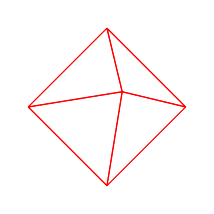
\begin{tikzpicture}[scale=3, line join=bevel, z=-5.5]
  \pic {octahedron};
\end{tikzpicture}

et avec la view définie aussi dans le préambule :

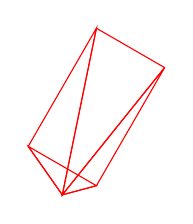
\begin{tikzpicture}[scale=3, view/isometric]
  \pic {octahedron};
\end{tikzpicture}
